\documentclass[a4paper,11pt]{article}
\usepackage[margin=2cm]{geometry}
%\usepackage{anysize}
\usepackage[pdftex]{graphicx}
\usepackage{url}
\usepackage{fixltx2e}
\usepackage{listings}
\usepackage{textcomp}
\usepackage{wrapfig}
\usepackage{color}
\usepackage{subfig}
\usepackage{fancyhdr}
\usepackage{newclude}
\usepackage[nodayofweek]{datetime}
\usepackage[small,compact]{titlesec}
\usepackage[pdfborder=0]{hyperref}
\longdate

\setlength{\parskip}{11pt} 
\setlength\parindent{0pt}

\pagestyle{fancyplain}
\fancyhf{}
\lhead{\fancyplain{}{Machine Learning CBC}}
\rhead{\fancyplain{}{\today}}
\cfoot{\fancyplain{}{\thepage}}


\title{395 Machine Learning\\\Large{--- Assignment 3 ---}}
\author{Group 7\\Porfyrios Vasileiou, Afxentios Hadjiminas, John Flanagan.\\
       \{pv311, ah2411, jf311.\}@doc.ic.ac.uk\\ \\
       \small{CBC helper: Ioannis Marras}\\
       \small{Course: CO395, Imperial College London}
}


\begin{document}
\maketitle

\section{CBR Case Implementation}

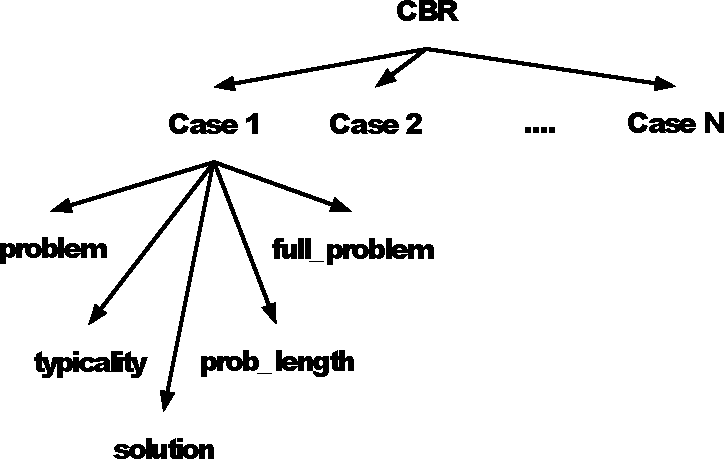
\includegraphics[width=.5\textwidth]{structure.pdf}

\section{CBR System Implementation}

\subsection{Retrieve Function}

\subsection{Reuse  Function}

\subsection{Retain  Function}

\section{Similarity Measures}

\subsection{Euclidean}

\subsection{Manhattan}

\subsection{Chebyshev}

\section{Overall Results}

\subsection{Precision and Recall Per Fold}

\subsection{Performance(F1Measure) Per Fold}
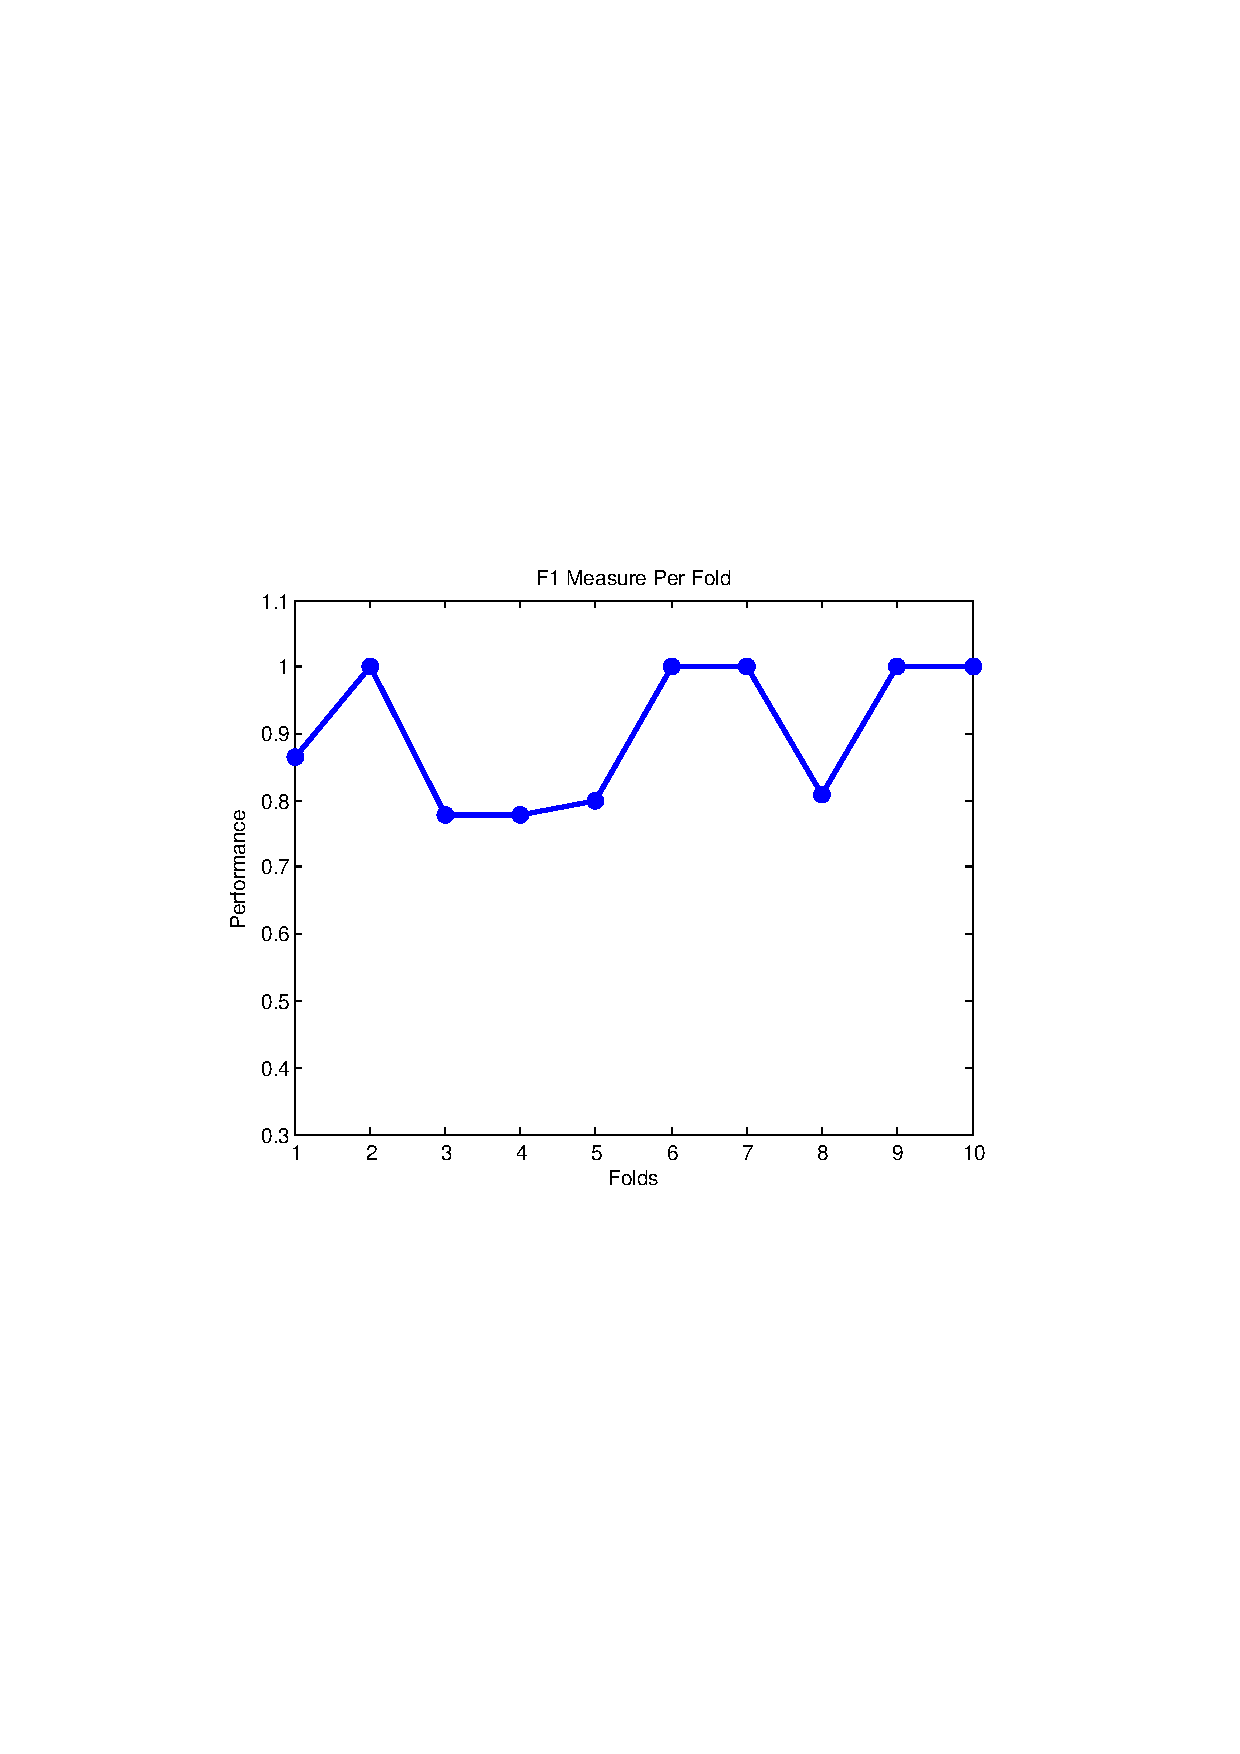
\includegraphics[width=.5\textwidth]{measure_per_fold.pdf}

\subsection{Average Confusion Matrix}

\subsection{Average Precision Recall F1Measure}


                                                             
% \begin{center}                                                                  
     % \begin{tabular}{ | l || c | c | c | c | c | c | }                           
     % \hline                                                                      
           % & Anger 1 & Disgust 2 & Fear 3 & Happiness 4 & Sadness 5 & Surprise 6 \\ \hline \hline
         % Anger 1 		& 11 & 0 & 1 & 0 & 0 & 0 \\ \hline                               
         % Disgust 2 		& 1 & 21 & 0 & 0 & 0 & 0 \\ \hline                            
         % Fear 3 		& 2 & 0 & 5 & 0 & 0 & 0 \\ \hline                                
         % Happiness 4 	& 0 & 1 & 0 & 23 & 0 & 0 \\ \hline                          
         % Sadness 5 		& 1 & 0 & 0 & 0 & 11 & 0 \\ \hline                             
         % Surprise 6 	& 0 & 0 & 0 & 0 & 0 & 23 \\ \hline                           
     % \end{tabular}                                                               
     % \\ Six Single-Output Confusion Matrix.                                              
% \end{center}                                                                    

                                                              
 % \begin{center}                                                                  
 % \begin{tabular}{ | l || c | c | c | c | c | c | }                               
     % \hline                                                                      
           							% & Anger 1 & Disgust 2 & Fear 3 & Happiness 4 & Sadness 5 & Surprise 6 \\ \hline \hline
         % Avg Recall 				& 0.9167 & 0.9545 & 0.7143 & 0.9583 & 0.9667 & 1 \\ \hline   
         % Avg Precision 				& 0.7333 & 0.9545 & 0.8333 & 1 & 1 & 1 \\ \hline
         % F\textsubscript{1} Measure & 0.8148 & 0.9545 & 0.7692 &  0.9787 &  0.9565 & 1 \\ \hline
     % \end{tabular}                                                               
     % \\ Six Single-Output evaluation results                                                                                               
 % \end{center}                                                                    


\end{document}
